\documentclass[journal]{IEEEtran}

\usepackage[utf8]{inputenc}
\usepackage[T1]{fontenc}
\usepackage[spanish,es-noquoting,es-nodecimaldot]{babel}
\usepackage{amsmath}
\usepackage{graphicx}
\usepackage{booktabs}
\usepackage{url}
\usepackage{float}

\begin{document}

\title{Modelo predictivo de riesgo de mora en contratos de leasing de motocicletas\\
\large Proyecto de aula, Modelos y Simulación de Sistemas II: Entregable II}

\author{Juan Esteban Cardozo Rivera, Maria Carolina Cardona Calderon y Oliver Andres Quiroz Mora%
\thanks{Departamento de Ingeniería de Sistemas, Universidad de Antioquia, Colombia. Grupo 14.}}

\maketitle

% =====================================================================
\section{Introducción}

Este documento presenta el desarrollo del modelo en dos etapas descrito en el Entregable I: una primera etapa no supervisada que identifica perfiles de comportamiento de pago y una segunda etapa supervisada que estima la probabilidad de que un contrato de leasing de motocicletas termine en riesgo grave de mora. Atiende además la retroalimentación recibida sobre el primer entregable, que pedía validar de forma temporal y no aleatoria, evitar la fuga de información entre las etapas, justificar la etiqueta con un criterio de negocio, analizar la sensibilidad de los parámetros de ventana y reportar más métricas por clase. El detalle completo de las variables y de cada experimento se encuentra en los cuadernos de código que acompañan al informe (cuadernos 01 a 05); aquí se resume el razonamiento y se muestran los resultados principales.

% =====================================================================
\section{Estado del arte}

La calificación por comportamiento (\emph{behavioural scoring}) estima la probabilidad de que un cliente que ya tiene un crédito incumpla en un horizonte definido, a partir de su historial de pagos. Se aborda casi siempre como clasificación binaria supervisada, y dos de los cuatro trabajos revisados anteponen una etapa no supervisada que agrupa a los clientes y entrega ese grupo al clasificador \cite{yuan2022,bakoben2020}, la misma arquitectura que adopta este proyecto. Ninguno de los cuatro valida con una partición estrictamente temporal de principio a fin ni prueba el modelo en una población distinta de aquella con la que se entrenó, dos aspectos que sí se cubren aquí.

Yuan et al. \cite{yuan2022} predicen el incumplimiento de 3.425 empresas chinas cotizadas (521 en default, una proporción cercana a 1:6) hasta cinco años antes. Agrupan las empresas con k-means y entrenan en cada grupo un clasificador de una sola clase, la descripción de dominio con vectores de soporte (SVDD), que ajusta una hiperesfera alrededor de la clase mayoritaria. Eligen los hiperparámetros con validación cruzada de cinco pliegues sobre el 80~\% de los datos y evalúan en el 20~\% restante. Reportan un AUC de entre 85~\% y 90~\% en los cinco horizontes y concluyen que el modelo de dos etapas supera a los de una sola etapa, aunque su ventaja se reduce en bases pequeñas, lo cual es relevante para una muestra como la nuestra. Se parece a este proyecto en la arquitectura de dos etapas; se diferencia en que predice empresas con estados financieros y no clientes con historial de pagos, y en que su evaluación es una partición única al azar.

Bakoben et al. \cite{bakoben2020} trabajan con 494 cuentas de tarjeta de crédito de un banco del Reino Unido, con 27,3~\% de cuentas en default tras sub-muestrear los buenos pagadores. Resumen el comportamiento mensual de cada cuenta con los coeficientes de un modelo autorregresivo vectorial de primer orden, agrupan con k-medoids usando una disimilitud que tiene en cuenta la incertidumbre de esos coeficientes y emplean el grupo como único predictor en una regresión logística. Evalúan con 1.000 particiones aleatorias 60/40. En la tarea de predicción el AUC es de 0,764, con H-measure de 0,375 y KS de 0,544, frente a 0,531 del modelo que solo usa promedios del comportamiento y a 0,678 cuando el agrupamiento ignora la incertidumbre. En la tarea de pronóstico, donde los grupos se arman con el primer tramo del historial y el incumplimiento se mide en el último, el AUC baja a 0,725, con H-measure de 0,183 y KS de 0,338. Es el antecedente más cercano a este proyecto, pues separa una ventana de observación de una de pronóstico y no usa la morosidad para agrupar. Se diferencia en que allí el perfil por sí solo logra casi todo el poder predictivo, mientras que en nuestros datos el perfil no mejora a un clasificador que ya recibe las variables que lo definen, y en que su muestra es pequeña y su partición, aleatoria.

Kennedy et al. \cite{kennedy2013} estudian con regresión logística con regularización ridge, sobre 2.500 hipotecas irlandesas, cómo cambia la dificultad de la tarea con la longitud del historial usado (6, 12 y 18 meses), con el horizonte de predicción (de 3 a 24 meses) y con la definición de moroso (atraso medido al final del horizonte o en cualquier momento de este). Entrenan con cuentas abiertas en 2003 y prueban fuera de tiempo con cuentas de 2004, y encuentran que un historial de 12 meses es el más fácil de predecir, que el desempeño cae claramente cuando el horizonte supera los seis a doce meses y que definir la mora como un atraso en cualquier momento del horizonte facilita la clasificación. Respaldan así la elección de una etiqueta definida sobre toda la ventana de predicción y la necesidad de analizar la sensibilidad a la longitud de las ventanas, que en este proyecto se hace con una rejilla de valores. Se diferencian en que su problema es hipotecario y mensual, y en que no incluyen una etapa no supervisada.

Ala'raj et al. \cite{alaraj2021} proponen una red LSTM bidireccional con atención, que recibe la secuencia de seis meses de pagos de 30.000 clientes de tarjeta de crédito de Taiwán, con 22~\% de morosos. La comparan con gradient boosting, una red neuronal con bagging, SVM, random forest y regresión logística mediante validación cruzada de cinco pliegues aleatorios. La LSTM obtiene una exactitud de 82,4~\%, una sensibilidad de 37,5~\%, una especificidad de 95,2~\%, un AUC de 78,5~\%, un puntaje de Brier de 13,3~\%, un KS de 0,43 y un H-measure de 0,30, y la prueba de McNemar indica que sus diferencias con los demás modelos son significativas. Pero gradient boosting queda muy cerca, con 78,0~\% de AUC, mientras que la regresión logística llega a 71,8~\% y el SVM a 69,6~\%, y todos los modelos detectan menos del 40~\% de los morosos con el umbral por defecto. Se parece a este proyecto en el orden de magnitud del AUC y en la dificultad de detectar la clase minoritaria; se diferencia en que no hay etapa de agrupamiento y en que sus pliegues aleatorios no respetan el orden del tiempo.

En conjunto, la literatura respalda la arquitectura de dos etapas y la necesidad de fijar con claridad las ventanas y la definición de mora, y muestra que con historiales cortos los métodos de ensamble rinden casi igual que las redes profundas. Las métricas que reportan van más allá de la exactitud e incluyen el AUC, el KS, el H-measure, el puntaje de Brier y, en el caso del desbalance, la media geométrica y el error tipo II. Para este proyecto se adoptan el AUC, el F1 de cada clase, la exactitud balanceada, la media geométrica y el coeficiente de correlación de Matthews, además de la precisión en el grupo de mayor riesgo, que refleja el uso real del modelo. No se reportan el KS, el H-measure ni el puntaje de Brier que no figuran entre las métricas del curso.

% =====================================================================
\section{Definición del problema y de la etiqueta}

La unidad de análisis es el episodio: un cliente con una moto, identificado por el contrato y su fecha de inicio, porque el número de contrato identifica la motocicleta y se reasigna entre clientes. El estudio se limita a Cartagena para el entrenamiento, y las sedes de Sincelejo y Montería se usan al final como población de validación externa. Para cada episodio, el momento de la predicción es el final de la semana 8, y la ventana de predicción comprende las semanas 9 a 20.

Un episodio está en riesgo grave de mora si alguna cuota que vence en la ventana de predicción alcanza 14 o más días de atraso, o si nunca se pagó porque el episodio terminó con una carta de retiro por mal comportamiento. Catorce días equivalen a dos cuotas semanales vencidas: un atraso aislado puede ser un descuido, mientras que dos cuotas seguidas sin pagar ya constituyen un patrón. La empresa no tiene una regla formal para el umbral, porque el cobro y el retiro quedan al criterio de cada supervisor, de modo que esta es una definición operativa del equipo y no una política de la empresa. Para no depender de esa elección, se repite el análisis con umbrales de 7 y 21 días, y el desempeño se mantiene en el mismo rango: con ocho semanas de observación y doce de predicción, el AUC de validación es de 0,775 con 7 días, 0,805 con 14 y 0,790 con 21, y el de prueba, de 0,775, 0,756 y 0,758. El retiro de la moto es una decisión discrecional de la empresa y por eso no se usa como etiqueta, sino solo como evidencia de validación y para decidir si una cuota nunca pagada al cierre cuenta como evento.

La corrección de la etiqueta respecto al primer entregable consiste en que los episodios cerrados con una cuota sin pagar, con menos de 14 días de atraso al cierre y sin carta de retiro por mal comportamiento, salen de la población, porque su desenlace no es observable: no hay evidencia de que el atraso hubiera sido grave ni de que no lo fuera. La población final tiene 2.889 episodios, de los cuales el 35,5~\% son positivos.

Las variables de entrada se calculan únicamente con la información disponible hasta el final de la semana 8. Una cuota vencida antes de ese momento y pagada después se trata como no pagada, con el atraso acumulado hasta esa fecha, porque es lo que la empresa sabría ese día. Describen el atraso (proporción de cuotas atrasadas, proporción con tres o más días de atraso, atraso promedio, cuotas sin pagar), el monto pagado (déficit relativo respecto a la cuota, pago total, variabilidad del pago), el esfuerzo de pago (pagos por cuota y días hasta el primer pago), las multas, las justificaciones de enfermedad o inmovilización y las características del contrato, que son la frecuencia de pago, la empresa, el día de vencimiento y la cuota. Los datos faltantes se imputan con la mediana junto con un indicador de ausencia, y todo ajuste de este tipo se hace solo con los datos de entrenamiento.

% =====================================================================
\section{Metodología}

La evaluación es temporal. Los episodios se ordenan por fecha de inicio y el 20~\% más reciente forma la prueba, que se usa una sola vez al final. El resto es el conjunto de desarrollo, donde se valida con pliegues de ventana expansiva: el modelo se entrena con lo anterior y se valida en el tramo siguiente. Se purgan los episodios cuya etiqueta se resuelve después del inicio de la prueba o del pliegue, para que ningún entrenamiento use información del futuro. Con el corte del 3 de diciembre de 2025, el desarrollo queda con 1.735 episodios (32,0~\% positivos), la prueba con 582 (38,7~\% positivos) y 572 episodios se purgan. Que la proporción de positivos suba con el tiempo, de 27~\% a 41~\% entre los pliegues, es la razón principal para validar por fecha y no al azar.

Para evitar la fuga de información entre las etapas, la imputación, el escalamiento, la codificación, el agrupamiento y cualquier selección de variables o reducción de dimensión forman parte de un mismo flujo que se reajusta en cada pliegue con sus datos de entrenamiento, y en validación y prueba solo se transforma. Las métricas son el AUC, el F1 de cada clase, la exactitud balanceada, la media geométrica y el coeficiente de correlación de Matthews. El umbral de decisión se elige maximizando la media geométrica sobre las predicciones de validación y se aplica sin cambios a la prueba. Los modelos se comparan por su AUC de validación, media de los pliegues, y la prueba solo informa.

% =====================================================================
\section{Resultados}

\subsection{Etapa 1: perfiles de comportamiento de pago}

El agrupamiento se hace con k-means sobre las variables de comportamiento de las primeras ocho semanas, sin usar la etiqueta. Se eligen cuatro perfiles por estabilidad: la estabilidad del agrupamiento, medida con el índice de Rand ajustado, es de 0,81 con cuatro perfiles y baja a 0,57 con cinco. Los métodos jerárquico y de mezclas gaussianas coinciden solo en parte con k-means (índice de 0,65 a 0,70), por lo que se conserva k-means por su simplicidad. Aunque la morosidad no interviene, los perfiles se ordenan por riesgo: en entrenamiento el porcentaje de episodios positivos es de 15, 29, 59 y 81~\% desde el perfil más puntual hasta el más atrasado, y en la prueba es de 19, 37, 74 y 73~\%, con solo 15 episodios en el último perfil de prueba. Este resultado indica que los perfiles son interpretables y tienen sentido de negocio, algo que ya apuntaba el trabajo de Bakoben et al. \cite{bakoben2020}. La Fig.~\ref{fig:perfiles} muestra el porcentaje de episodios con riesgo grave en cada perfil, tanto en el entrenamiento como en la prueba más reciente.
\begin{figure}[!t]
\centering
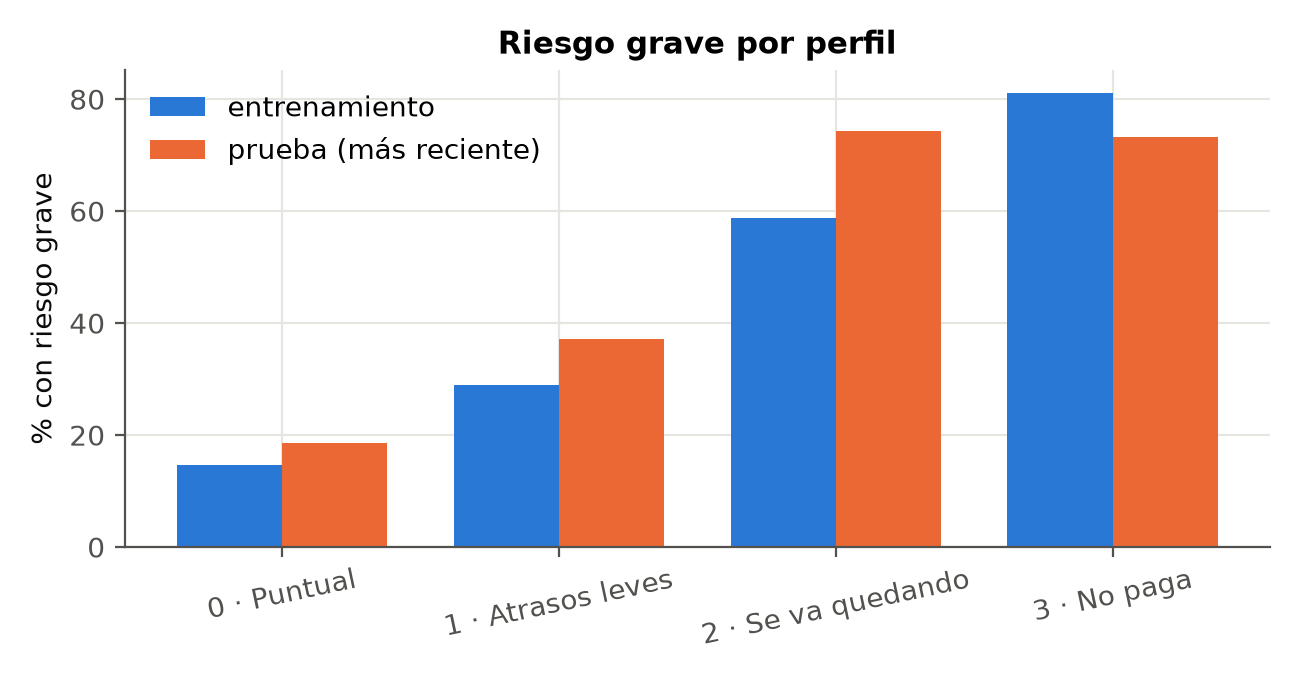
\includegraphics[width=\columnwidth]{figuras/riesgo_por_perfil.png}
\caption{Porcentaje de episodios con riesgo grave en cada uno de los cuatro perfiles de pago, en entrenamiento y en la prueba más reciente.}
\label{fig:perfiles}
\end{figure}


\subsection{Etapa 2: clasificación}

Se comparan seis clasificadores del curso: regresión logística, vecinos más cercanos, árbol de decisión, random forest, gradient boosting y máquina de vectores de soporte con núcleo gaussiano. El AUC de validación y de prueba es, respectivamente, de 0,805 y 0,756 para la regresión logística, de 0,798 y 0,784 para random forest, de 0,784 y 0,783 para gradient boosting, de 0,782 y 0,701 para los vecinos más cercanos, de 0,781 y 0,722 para la máquina de vectores de soporte y de 0,741 y 0,759 para el árbol. La regresión logística y random forest no se distinguen con claridad, pues su diferencia es menor que la desviación entre pliegues, que es de unos 0,02. Se toma la regresión logística como modelo base por su interpretabilidad: en la prueba alcanza un AUC de 0,756 (intervalo de confianza del 95~\%, de 0,72 a 0,79), una exactitud balanceada de 0,69, un F1 de 0,62 para la clase de riesgo y un coeficiente de Matthews de 0,37. El valor de 0,81 que se obtenía con una partición aleatoria era optimista. La Tabla~\ref{tab:modelos} resume todas las métricas de los seis modelos, la Fig.~\ref{fig:comparacion} compara su AUC en validación y en prueba, y la Fig.~\ref{fig:roc} muestra la curva ROC y la matriz de confusión del modelo base en la prueba: con el umbral elegido en validación, de los 225 episodios que realmente tuvieron riesgo grave se detectan 144, y se señalan 96 de los 357 que no lo tuvieron.
\begin{table}[!t]
\caption{Desempeño de los seis clasificadores. Validación: media de los pliegues temporales; el resto, en la prueba.}
\label{tab:modelos}
\centering
\scriptsize
\setlength{\tabcolsep}{3pt}
\begin{tabular}{@{}lcccccc@{}}
\toprule
Modelo & AUC val. & AUC prueba & F1 (0) & F1 (1) & BACC & MCC \\
\midrule
Regresión logística & 0,805 & 0,756 & 0,747 & 0,619 & 0,686 & 0,367 \\
Random forest & 0,798 & 0,784 & 0,792 & 0,623 & 0,703 & 0,421 \\
Gradient boosting & 0,784 & 0,783 & 0,783 & 0,611 & 0,693 & 0,399 \\
KNN & 0,782 & 0,701 & 0,767 & 0,591 & 0,676 & 0,361 \\
SVM (RBF) & 0,781 & 0,722 & 0,775 & 0,598 & 0,683 & 0,378 \\
Árbol de decisión & 0,741 & 0,759 & 0,797 & 0,520 & 0,657 & 0,376 \\
\bottomrule
\end{tabular}
\end{table}

\begin{figure}[!t]
\centering
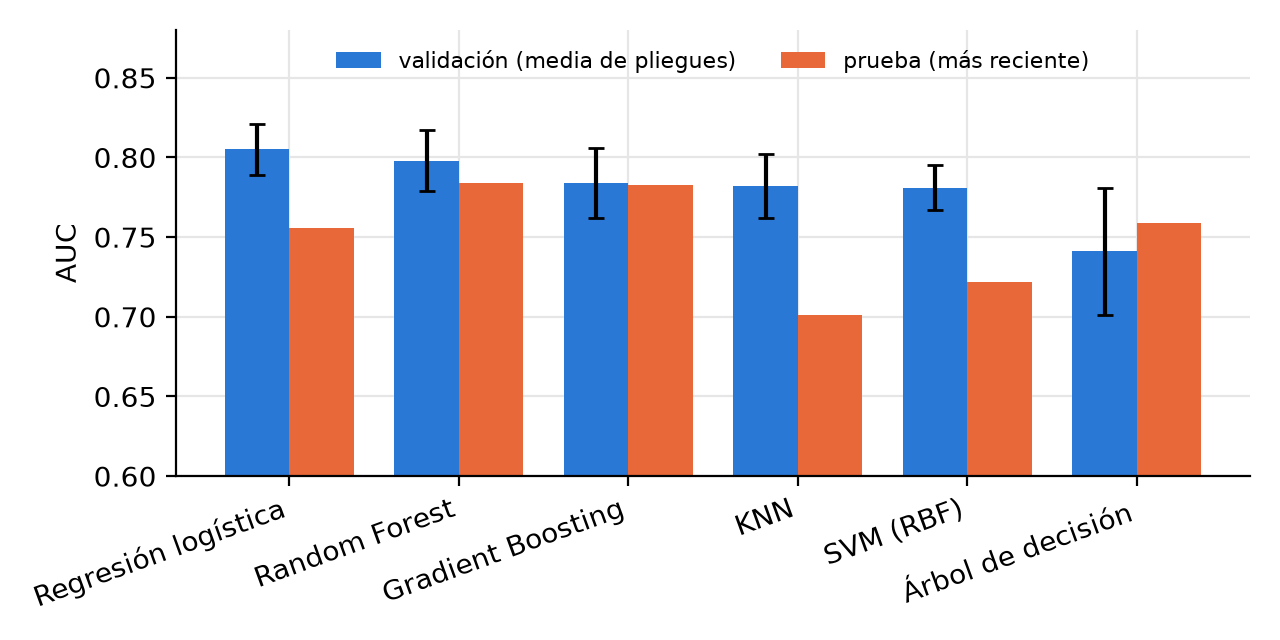
\includegraphics[width=\columnwidth]{figuras/comparacion_modelos.png}
\caption{AUC de los seis clasificadores en validación (media de los pliegues temporales y desviación) y en la prueba más reciente.}
\label{fig:comparacion}
\end{figure}

\begin{figure}[!t]
\centering
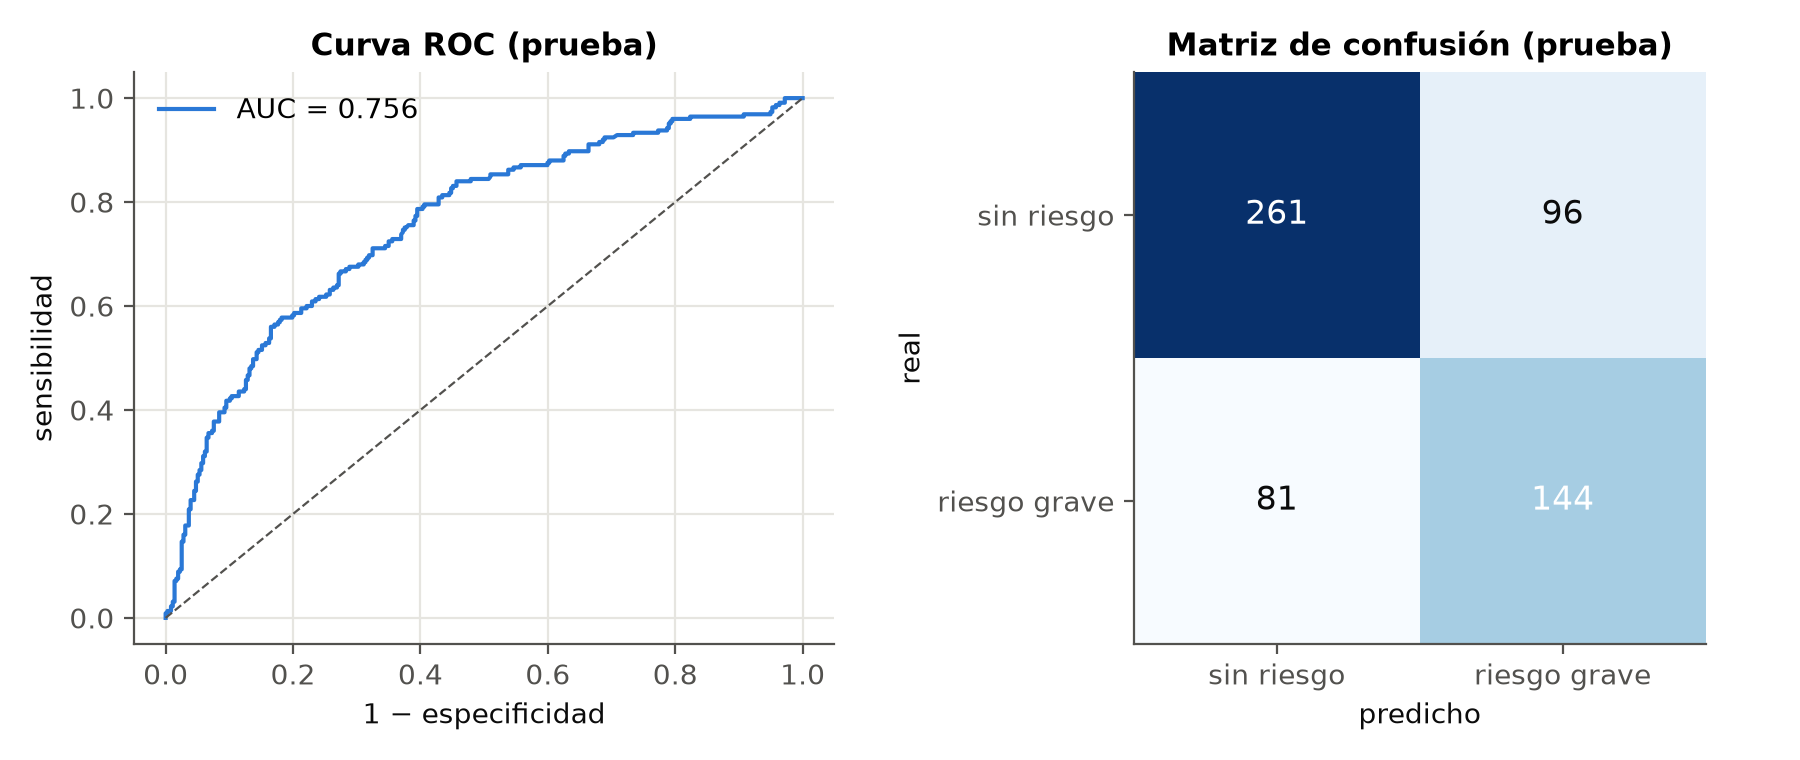
\includegraphics[width=\columnwidth]{figuras/modelo_final.png}
\caption{Curva ROC y matriz de confusión del modelo base (regresión logística) en la prueba.}
\label{fig:roc}
\end{figure}


Dos hallazgos van en contra de lo esperado. Primero, ni el perfil de la etapa 1 ni las marcas de gestión de la empresa mejoran al clasificador, con diferencias de AUC menores a 0,004, de modo que el perfil sirve para describir la cartera, pero no agrega información a quien ya conoce las variables que lo definen. Segundo, el tratamiento del desbalance, ya sea con ponderación de clases, submuestreo o SMOTE, no cambia el AUC, lo cual es razonable con un 35~\% de positivos.

\subsection{Sensibilidad a las ventanas y al umbral}

Se evaluó una rejilla de 36 combinaciones de semanas de observación (4, 6, 8 y 12), de semanas de predicción (8, 12 y 16) y de días de atraso (7, 14 y 21). Con cuatro semanas de observación se predice igual o mejor que con ocho; por ejemplo, con ocho semanas de predicción y 14 días, el AUC de validación es de 0,831 frente a 0,802. Un horizonte de 16 semanas rinde peor. Con doce semanas de observación el AUC de prueba es el más alto, de 0,85, pero es engañoso, porque cambia la población y quedan unos 500 episodios. Como cada combinación define una población distinta, los valores del AUC entre filas no son estrictamente comparables, y la rejilla debe leerse como una comprobación de robustez de la elección de ocho y doce semanas y no como un criterio para elegir los parámetros (Fig.~\ref{fig:rejilla}).


\begin{figure*}[!t]
\centering
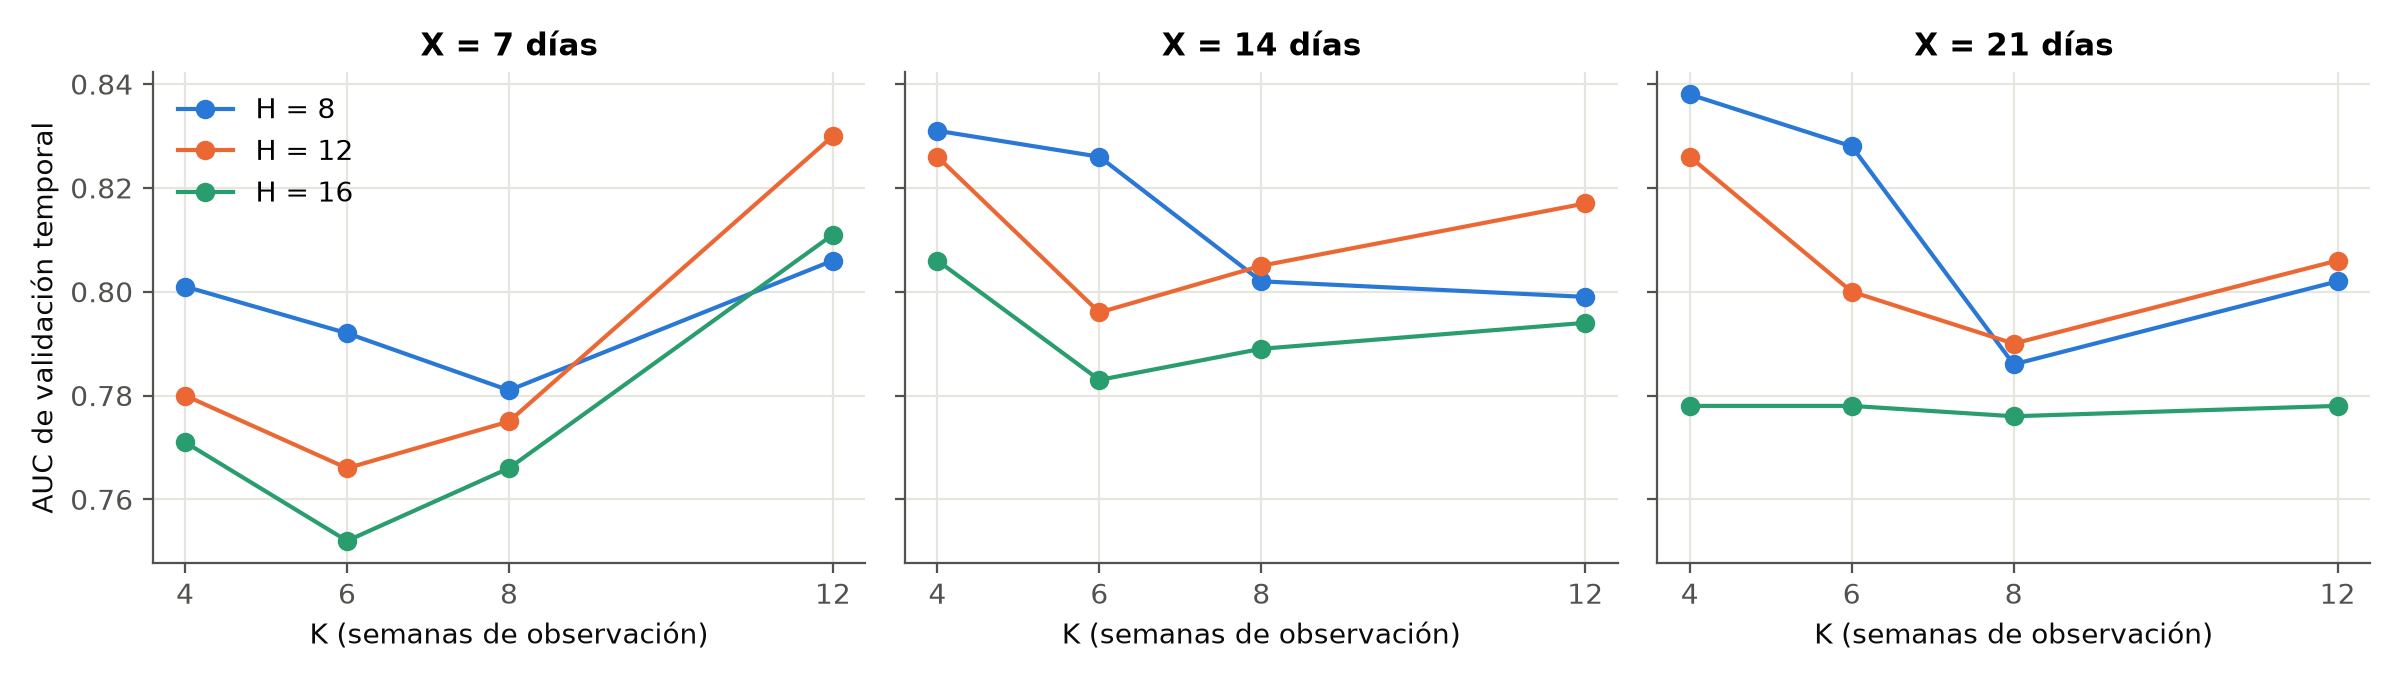
\includegraphics[width=\textwidth]{figuras/rejilla_khx.png}
\caption{AUC de validación temporal para las combinaciones de semanas de observación ($K$), semanas de predicción ($H$) y días de atraso ($X$).}
\label{fig:rejilla}
\end{figure*}

\subsection{Selección de variables y explicabilidad}

Las variables más asociadas con la etiqueta, medidas por el AUC de cada una por separado, son el atraso promedio (0,759), el déficit relativo (0,749), la proporción de cuotas atrasadas (0,731) y el pago total (0,727, con signo negativo). Con solo cinco variables elegidas por información mutua, el AUC de validación es de 0,788 frente a 0,809 con todas, de manera que el modelo puede simplificarse con poca pérdida. La reducción de dimensión no ayuda: el análisis de componentes principales necesita 10 de 28 componentes para explicar el 90~\% de la varianza sin mejorar la clasificación, y el uso de UMAP como entrada empeora el AUC a 0,665. Entre pliegues se mantiene un núcleo estable de variables: la proporción de cuotas con tres o más días de atraso, las cuotas sin pagar al momento de la predicción, la variabilidad del pago y el déficit relativo. En el análisis con valores de SHAP, después de la empresa, los factores de mayor peso son el déficit relativo, el atraso promedio y la proporción de cuotas con tres o más días de atraso. Un matiz que conviene tener presente es precisamente que la empresa (MotoHoy o RentaYa) encabeza ese ranking y pesa mucho en la regresión logística, y aún falta confirmar con la empresa que este campo sea confiable y qué distingue a los clientes de RentaYa. La Fig.~\ref{fig:shap} muestra cómo cada variable empuja la predicción: valores altos de déficit relativo, de atraso promedio y de cuotas sin pagar aumentan el riesgo estimado.
\begin{figure}[!t]
\centering
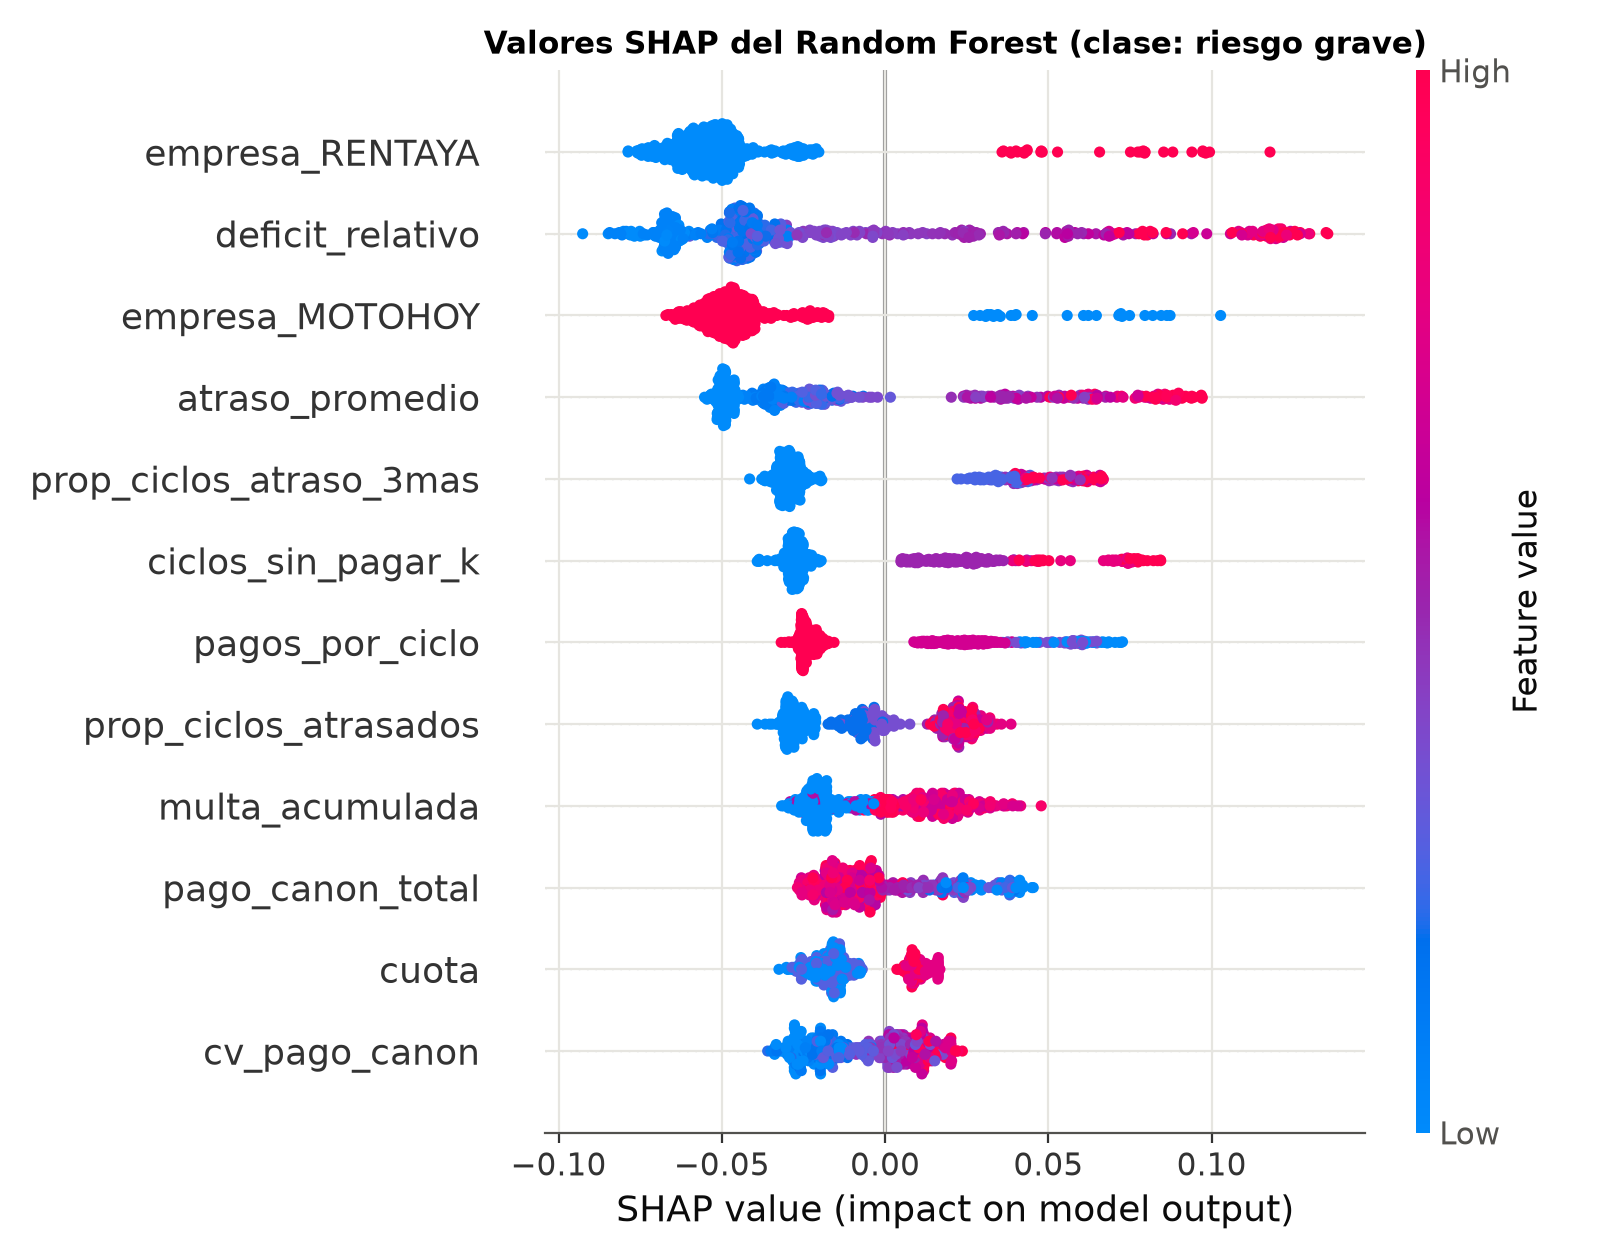
\includegraphics[width=\columnwidth]{figuras/shap_resumen.png}
\caption{Valores SHAP del random forest para la clase de riesgo grave: cada punto es un episodio, y el color indica si el valor de la variable es bajo (azul) o alto (rojo).}
\label{fig:shap}
\end{figure}


\subsection{Búsqueda de un mejor modelo}

Dado que seis algoritmos distintos quedan entre 0,78 y 0,80 de AUC de validación, se probaron cuatro vías para mejorar el resultado, todas con el mismo protocolo temporal. Se agregaron nueve variables de trayectoria que describen cómo termina la ventana de observación (el atraso de las últimas dos semanas, la tendencia y la desviación del atraso, el cambio entre la primera y la segunda mitad, los días desde el último pago, el mayor intervalo sin pagar y el dinero pagado en las últimas dos semanas), y los cambios de AUC quedaron dentro de la desviación entre pliegues. El ajuste de hiperparámetros con validación temporal solo subió el AUC de validación entre 0,002 y 0,005 en cada familia de modelos, con un máximo de 0,810 para la regresión logística penalizada, de 0,802 para random forest y de 0,790 para gradient boosting, y un ensamble por voto suave de regresión logística, random forest y gradient boosting llegó a 0,811 en validación y 0,788 en prueba, igual que random forest solo. Por último, se incorporaron, en modo de solo lectura, los registros de justificaciones y de gestión de cobranza anteriores a la semana 8 y se verificó con pruebas automáticas que los eventos posteriores no alteran las variables. Estas variables se asocian con la etiqueta, pero repiten lo que ya dicen los pagos y no mejoran la validación. La conclusión es que, con las primeras ocho semanas de información, el modelo está cerca de su máximo y que el límite proviene de la información de entrada y no del algoritmo (Fig.~\ref{fig:busqueda}).
\begin{figure}[!t]
\centering
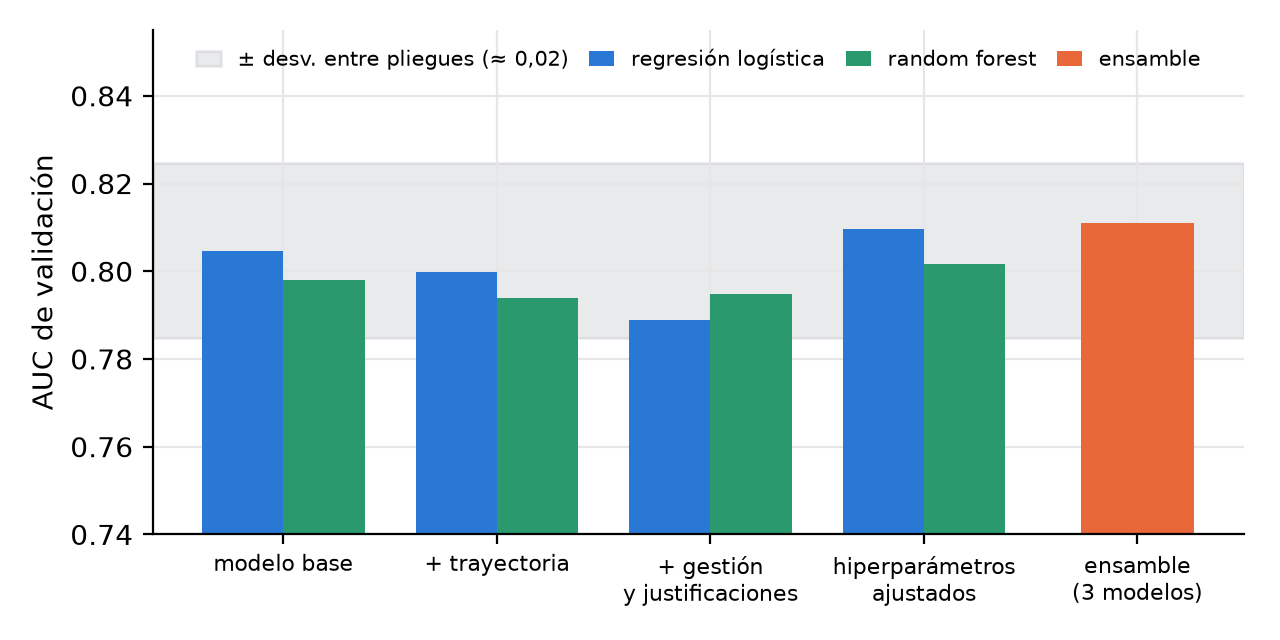
\includegraphics[width=\columnwidth]{figuras/busqueda_mejora.png}
\caption{AUC de validación del modelo base y de cada intento de mejora. La franja gris marca la desviación típica entre pliegues; ninguna variante sale de ella.}
\label{fig:busqueda}
\end{figure}


Una forma más cercana al uso real de medir el modelo es la precisión entre los episodios de mayor riesgo. Si la empresa revisara solo el 10~\% de los episodios de la prueba con mayor probabilidad, acertaría entre el 78~\% y el 79~\% de las veces según el modelo, frente a una tasa base de 38,7~\%, y entre el 74~\% y el 75~\% si revisara el 20~\%.

\subsection{Validación externa en otras sedes}

El modelo entrenado con todos los episodios de Cartagena se aplicó sin reajustarse a Sincelejo (793 episodios, 23,6~\% positivos) y Montería (199 episodios, 21,1~\% positivos), que usan la misma estructura de datos en servidores distintos y cuyo historial comienza a mediados de 2025 y a fines de ese año, respectivamente. En Sincelejo el AUC es de 0,767 con regresión logística, de 0,754 con random forest y de 0,761 con gradient boosting, y en Montería, de 0,783, 0,805 y 0,795. Son valores iguales o mayores que los de la prueba temporal de Cartagena, aunque la tasa de riesgo de las nuevas sedes es menor, y la precisión en el 10~\% de mayor riesgo es de 71 a 76~\% en Sincelejo y de 68~\% en Montería, unas tres veces la tasa base. Quitar la variable empresa cambia el AUC en menos de 0,003, porque en las sedes nuevas todos los episodios son de MotoHoy. El resultado de Montería se apoya en pocos episodios y tiene un margen de error amplio, por lo que la conclusión descansa sobre todo en Sincelejo. Como la tasa de riesgo cambia por sede, el umbral de decisión debería calibrarse para cada una (Fig.~\ref{fig:sedes}).
\begin{figure}[!t]
\centering
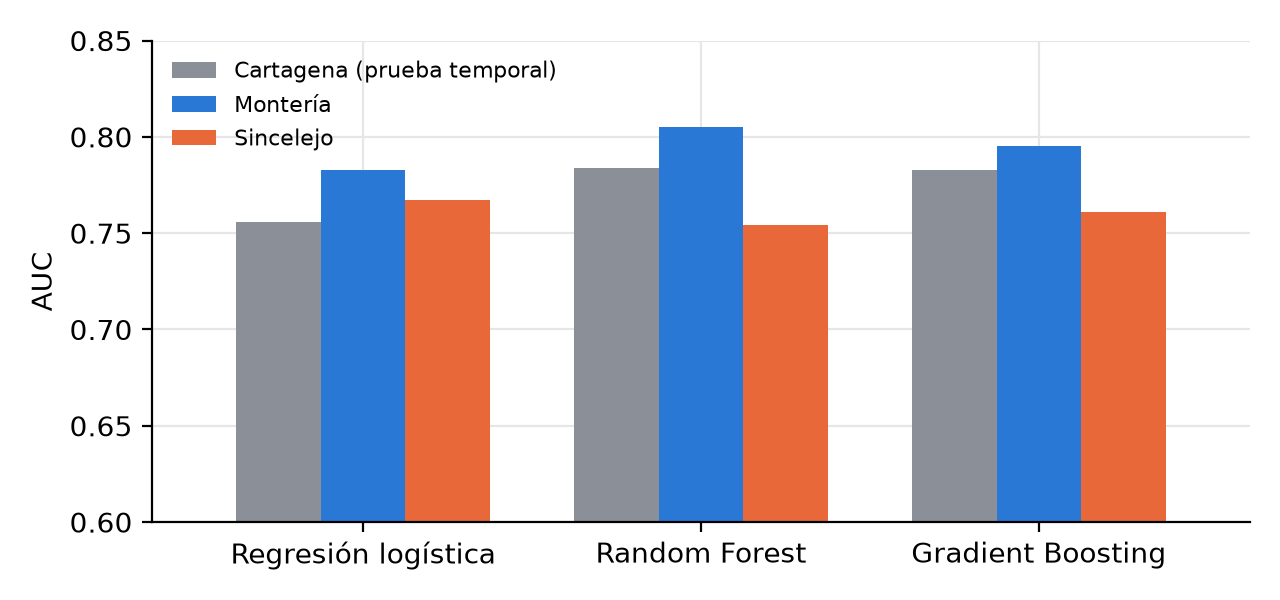
\includegraphics[width=\columnwidth]{figuras/validacion_sedes.png}
\caption{AUC de los tres mejores modelos, entrenados con Cartagena, al aplicarlos sin reajustar a Sincelejo y Montería, junto al AUC de la prueba temporal de Cartagena.}
\label{fig:sedes}
\end{figure}


% =====================================================================
\section{Limitaciones y conclusiones}

El resultado es un modelo que ordena los contratos por riesgo con un AUC cercano a 0,80 en validación y entre 0,76 y 0,79 en prueba, y que conserva ese desempeño en otras dos sedes sin reajustarse. No es un modelo que decida por sí solo ni reemplaza el criterio de los supervisores: sirve para priorizar la gestión temprana. Entre sus limitaciones están que la etiqueta se apoya en una definición operativa de 14 días, que la empresa no formaliza, y que el análisis de sensibilidad la respalda como robusta, pero no la valida como política; que el riesgo cambia con el tiempo, por lo que el modelo debe reentrenarse y su umbral recalibrarse periódicamente; que los retiros por mal comportamiento aportan 260 de los 1.026 positivos, y que una definición más estricta que los excluyera bajaría la proporción de positivos a cerca del 27~\%; y que la muestra de Montería es pequeña. Como trabajo futuro quedan la comprobación de la variable empresa con el equipo de cartera, la validación de la etiqueta con las cartas de retiro y una prueba de uso real en la que se compare la gestión con y sin la lista de contratos priorizados.

% =====================================================================
\begin{thebibliography}{4}

\bibitem{yuan2022}
K. Yuan, G. Chi, Y. Zhou y H. Yin, ``A novel two-stage hybrid default prediction model with k-means clustering and support vector domain description,'' \emph{Research in International Business and Finance}, vol.~59, art.~101536, 2022, doi: 10.1016/j.ribaf.2021.101536.

\bibitem{bakoben2020}
M. Bakoben, T. Bellotti y N. Adams, ``Identification of credit risk based on cluster analysis of account behaviours,'' \emph{Journal of the Operational Research Society}, vol.~71, no.~5, pp.~775--783, 2020, doi: 10.1080/01605682.2019.1582586.

\bibitem{kennedy2013}
K. Kennedy, B. Mac Namee, S. J. Delany, M. O'Sullivan y N. Watson, ``A window of opportunity: Assessing behavioural scoring,'' \emph{Expert Systems with Applications}, vol.~40, no.~4, pp.~1372--1380, 2013, doi: 10.1016/j.eswa.2012.08.052.

\bibitem{alaraj2021}
M. Ala'raj, M. F. Abbod y M. Majdalawieh, ``Modelling customers credit card behaviour using bidirectional LSTM neural networks,'' \emph{Journal of Big Data}, vol.~8, art.~69, 2021, doi: 10.1186/s40537-021-00461-7.

\end{thebibliography}

\end{document}
